\section{Overview and Implementation Plan}
This section explains how the Students\&Companies (S\&C) platform will be built, integrated, and tested. The development will happen in phases to ensure that each part of the system is created and tested individually before being connected to the rest. This way, problems can be caught early, and we can avoid larger issues later on.

The implementation will use a combination of two approaches:
\begin{itemize}
    \item  \textbf{Bottom-up} – We’ll start by developing and testing the essential features of the systems that do not require other functionalities to work.
    \item \textbf{Thread-based} – Once the core features are in place, we’ll add new features in parallel. This keeps development moving quickly and gives stakeholders something tangible to see along the way.
\end{itemize}

By using this hybrid method, different teams can work on separate features at the same time, integrating them as soon as they are ready. This not only speeds up development but also reduces the risk of big issues when the full system comes together.

Continuous feedback from stakeholders will be crucial throughout development.

\textbf{Alpha Testing} will be conducted internally by developers and select testers to identify major bugs early in the process. \textbf{Beta Testing} will involve releasing the platform to a limited audience to gather real-world feedback before full deployment.

During the testing phases, logs and reports will be collected to track issues, prioritize fixes, and improve overall system stability. This iterative approach ensures that the platform evolves based on real user interactions, allowing the team to fine-tune the system progressively.

\section{Features Identification}
The system's core features are extracted from the functional and non-functional requirements outlined in the RASD document. These features define how users will interact with the system and how different components will work together to provide a seamless experience. Below is a breakdown of the main features that will be developed, integrated, and tested to ensure the platform meets user expectations and operates smoothly.

\paragraph{[F1] User Authentication (Sign-up, Login, Logout).} This is one of the fundamental features of the platform. It allows users to create an account, log in, and log out securely. Authentication is essential for accessing any part of the system, ensuring that users' data is protected and only authorized individuals can perform specific actions. The platform will support multiple user roles, including students, companies, and university staff, each with different levels of access and privileges. Testing this feature will focus not only on the correctness of login and registration flows but also on ensuring that users are assigned the appropriate role and that permissions are strictly enforced.

\paragraph{[F2] Profile Management.} The profile management feature allows users to build and maintain detailed profiles, which serve as their digital resumes on the platform. Students can input information about their education, skills, and experiences, while companies can create organizational profiles showcasing their internship programs and job opportunities. Profile data is critical for the recommendation system, as it helps match students to internships that align with their qualifications and interests. Companies will also need access to student profiles to evaluate potential candidates during the recruitment process. Testing this feature will focus on ensuring that users can easily create and update their profiles, with real-time validation to prevent errors.

\paragraph{[F3] Internship Management.} This feature allows companies to create, edit, and delete internship listings. Students can search for opportunities based on various filters (location, required skills, etc.) and apply directly through the platform. When an internship is created or updated, the system will automatically notify relevant students who match the internship criteria. This ensures that companies can quickly find suitable candidates and that students do not miss out on potential opportunities. Testing will ensure that internships are properly stored in the database, updates are reflected in real-time, and notifications are sent without delays.

\paragraph{[F4] Recommendation System.} The recommendation system is designed to automate the matching process between students and internships. Using specialized algorithms, the system analyzes student profiles, resumes, and preferences to suggest relevant internship opportunities. This feature reduces the manual effort required from both students and companies, improving the efficiency and accuracy of the recruitment process. The recommendation engine will continuously learn from user interactions and feedback, refining its suggestions over time. Testing this feature will involve simulating different user scenarios to verify that the recommendations are accurate and relevant. Additionally, stress testing will be conducted to ensure the recommendation engine performs well under heavy loads.

\paragraph{[F5] Interview and Task Management.} This feature allows companies to create tasks, assign them to candidates, and evaluate their performance as part of the interview and selection process. Tasks can range from coding challenges to written assignments, providing companies with deeper insights into candidates' abilities. Students receive notifications when tasks are assigned and can submit their work directly through the platform. Companies can then review submissions, score them, and make final selections based on performance. Testing will ensure that tasks are correctly assigned, deadlines are enforced, and submissions are stored securely. The system will also be tested for scalability, as companies may assign tasks to multiple candidates simultaneously.

\paragraph{[F6] Feedback and Complaints.} After internships are completed, students and companies can provide feedback on their experiences. This feedback loop helps improve the matching process by refining the recommendation algorithm and providing valuable insights to users. Additionally, the platform allows users to file complaints if issues arise during an internship. Complaints are forwarded to university staff, who can mediate and work towards resolving disputes. Testing this feature will involve validating the feedback forms, ensuring data integrity, and verifying that complaints are routed to the appropriate parties without delays.

\paragraph{[F7] Notification System.}  The notification system keeps users informed about important events, such as new internship postings, application updates, interview invitations, and complaint resolutions. Notifications will appear within the platform and can also be sent via email for critical actions. This feature ensures that users remain engaged and do not miss essential updates. Testing will focus on the timeliness and accuracy of notifications, ensuring that they trigger correctly based on user actions and system events.

\newpage
\section{Integration Strategy}
The integration process will follow a progressive bottom-up approach, starting with basic infrastructure and culminating in full system integration. Each integration phase will involve component validation to ensure smooth communication between modules. We assume that WebApp, Web Server and DBMS are already tested and working.

\textbf{Phase 1 – Core Infrastructure:} Integrate the WebApp, Web Server, and DBMS to establish basic user interaction and start testing the Model and the Dashboard Manager with proper drivers.

\begin{figure}[H]
    \begin{center}
        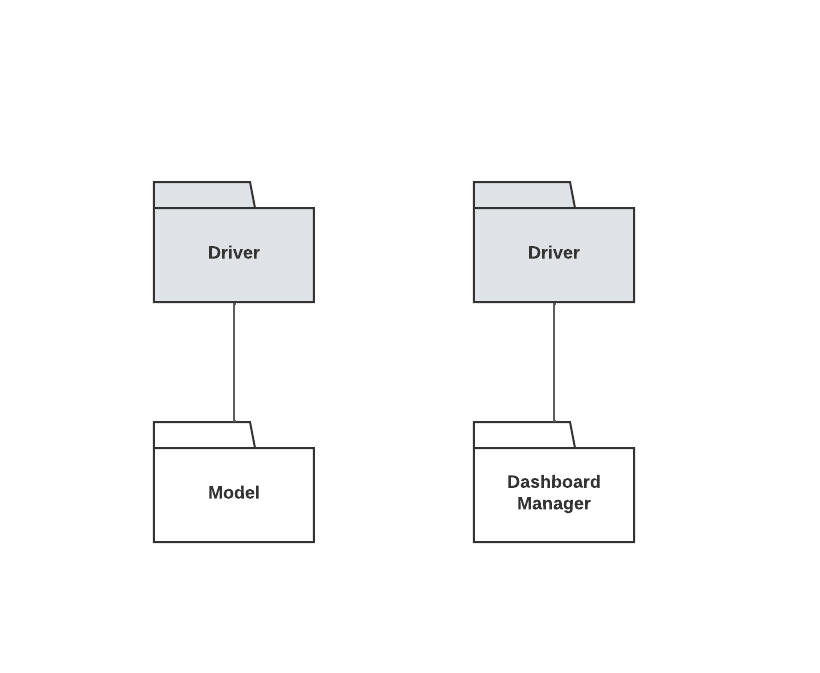
\includegraphics[width=0.5\linewidth]{Integration/Phase1.png}
        \label{fig:Integration_1}%
    \end{center}
\end{figure}

\textbf{Phase 2 – Profile and User Management:} Connect the Login Manager, Registration Manager and Profile Manager to the core system. Test operations on user profiles.

\begin{figure}[H]
    \begin{center}
        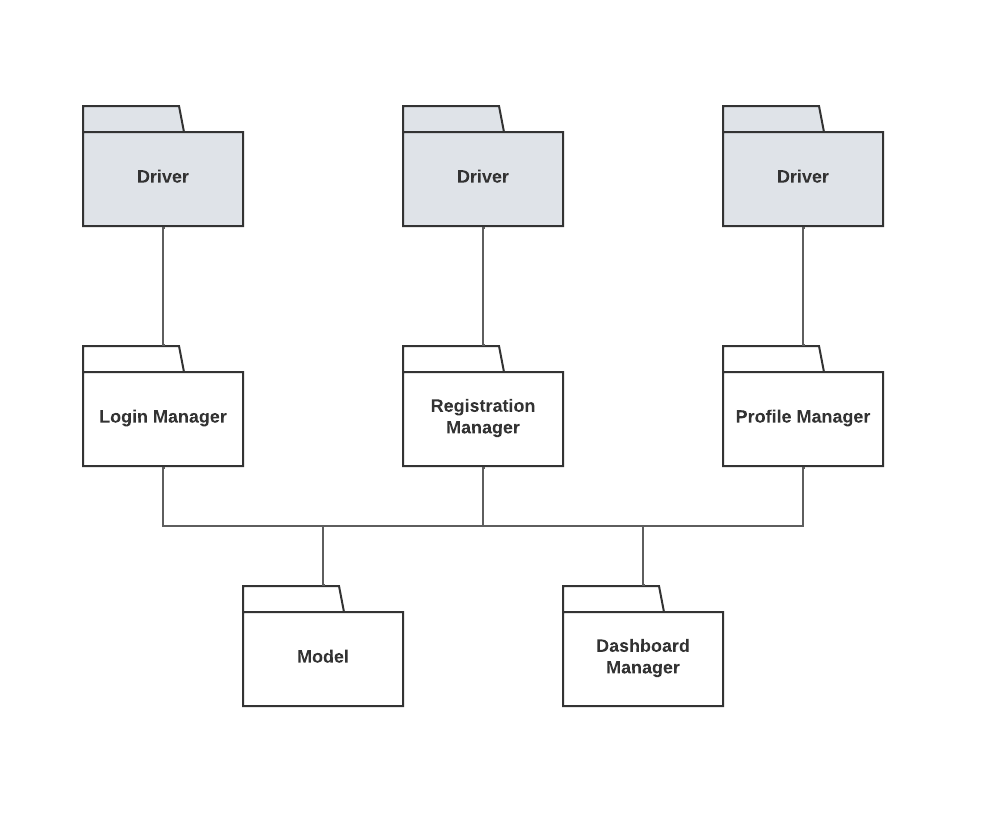
\includegraphics[width=0.6\linewidth]{Integration/Phase2.png}
        \label{fig:Integration_2}%
    \end{center}
\end{figure}

\textbf{Phase 3 – Internship and Application modules:} Incorporate the Internship Manager and Application Manager to enable internship creation and application. Test the end-to-end workflow, from internship posting to candidate application. Test the full interview cycle, from task creation to candidate evaluation.

\begin{figure}[H]
    \begin{center}
        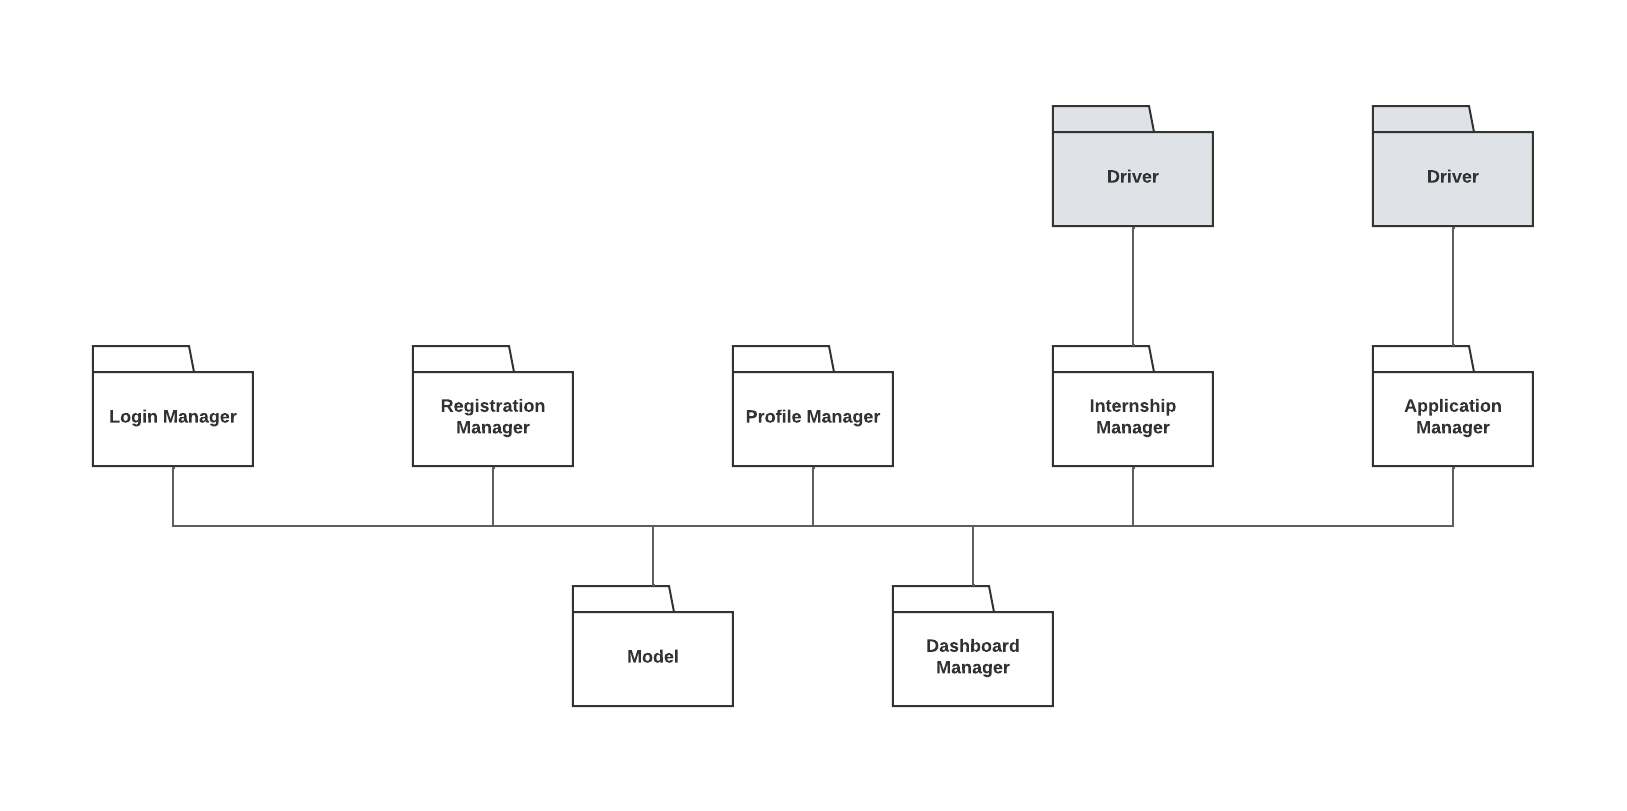
\includegraphics[width=0.9\linewidth]{Integration/Phase3.png}
        \label{fig:Integration_3}%
    \end{center}
\end{figure}

\textbf{Phase 4 – Recommendation and Complaints Systems:} Integrate the Recommendation Manager, linking it to the external tools for algorithm execution. Validate recommendation accuracy and matching efficiency. At the same time, another team can integrate the Complaints Manager, allowing users to submit complaints. Test communication channels between students, companies, and universities

\begin{figure}[H]
    \begin{center}
        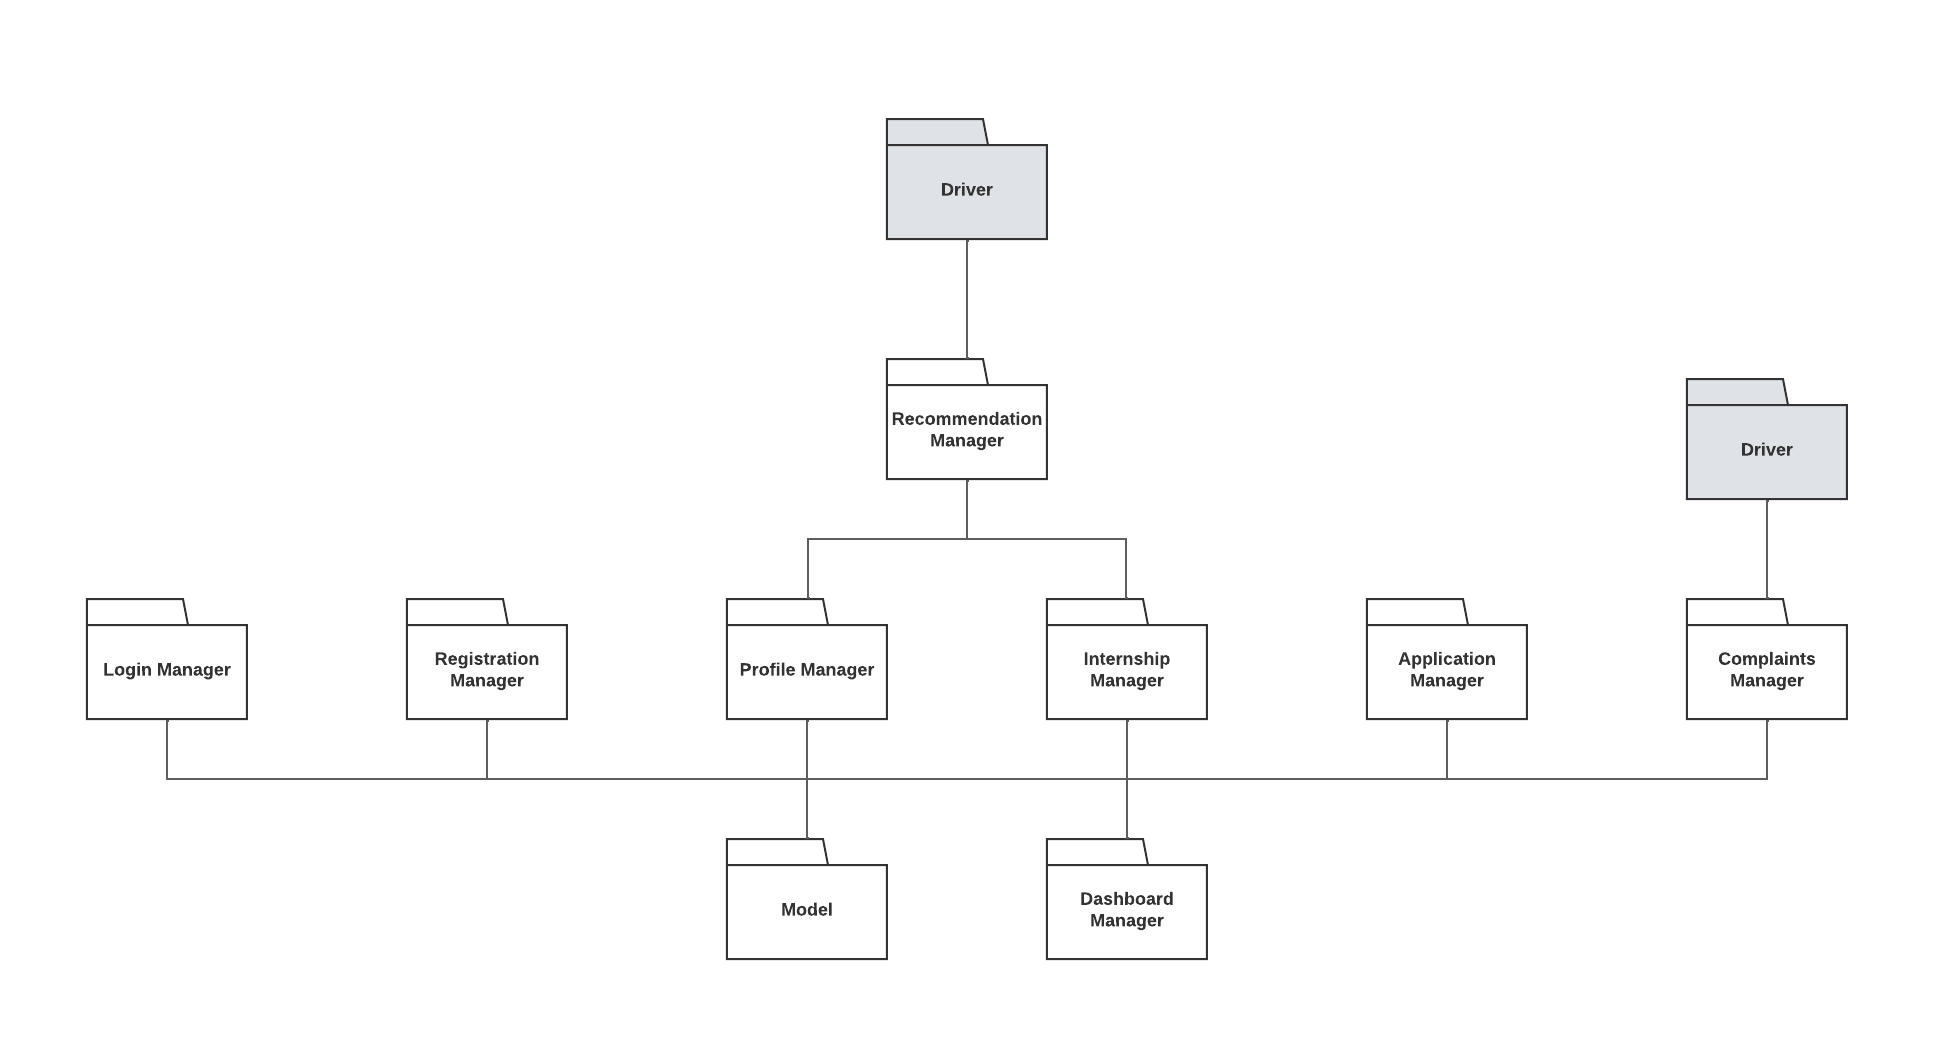
\includegraphics[width=0.9\linewidth]{Integration/Phase4.png}
        \label{fig:Integration_4}%
    \end{center}
\end{figure}

\textbf{Phase 5 – Notification System:} Integrate the Notification Manager, allowing the system to notify users. Test different types of notification coming from the system.

\begin{figure}[H]
    \begin{center}
        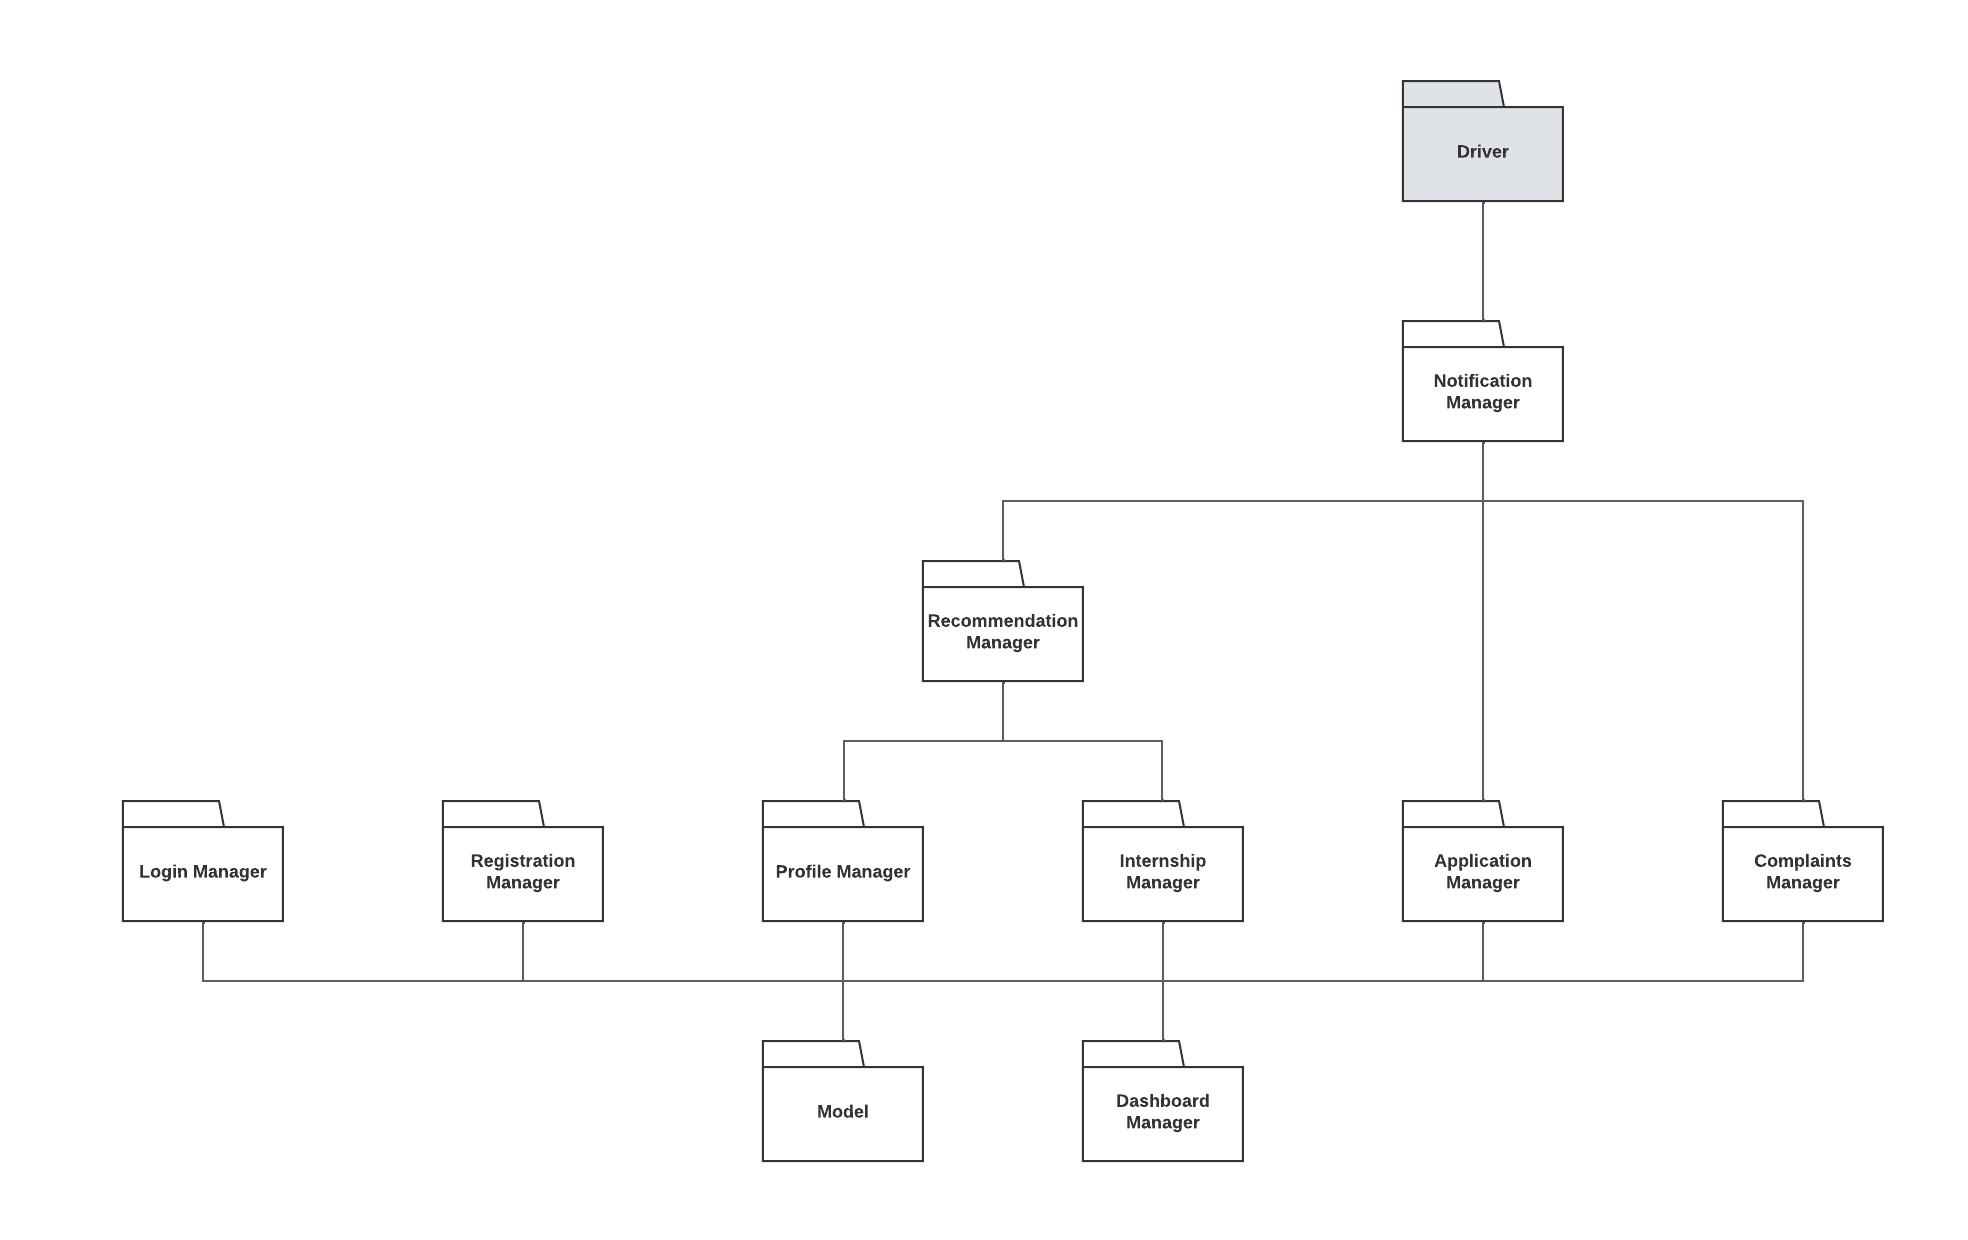
\includegraphics[width=0.9\linewidth]{Integration/Phase5.png}
        \label{fig:Integration_5}%
    \end{center}
\end{figure}

\textbf{Phase 6 – Full System Integration:} Connect all components into a fully functional system. Perform load and stress tests to assess scalability and performance.

\begin{figure}[H]
    \begin{center}
        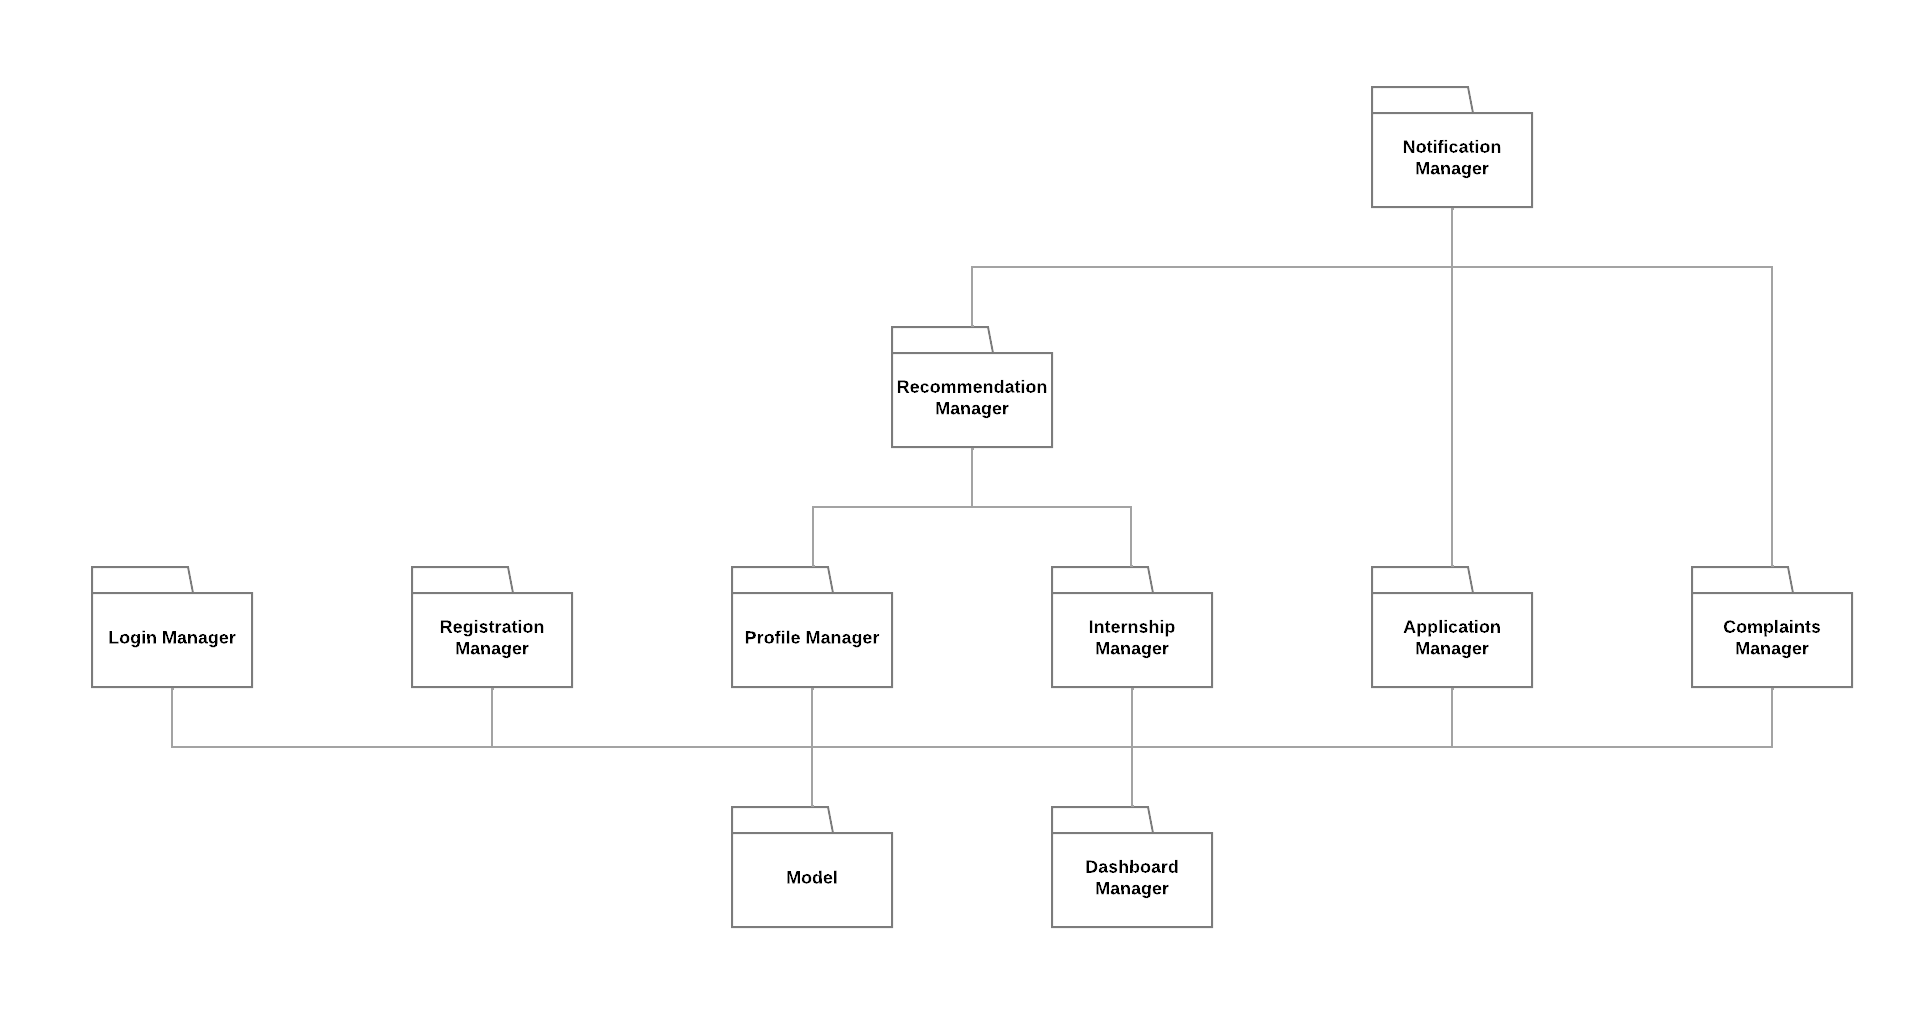
\includegraphics[width=1\linewidth]{Integration/Phase6.png}
        \label{fig:Integration_6}%
    \end{center}
\end{figure}

\section{System Testing Strategy}
After testing individual components to verify functionalities in isolation through the use of drivers that simulate the behaviour of missing components (unit testing) they will be progressively integrated with the rest of the system. After integration, a new driver will verify that the module not only operates as intended but also interacts correctly with the existing components. This incremental testing approach helps maintain system stability and ensures that the workflow remains consistent throughout development. After full integration of all components, system tests will be ran to verify the overall workflow, detect bugs, and confirm that the platform adheres to the functional and non-functional requirements outlined in the RASD document.
The following types of tests will be applied to validate the platform:

\begin{itemize}
    \item \textbf{Functional Testing:} Ensures that the platform behaves as described in the RASD by simulating real-world workflows. This includes validating user actions like authentication, internship applications, and task submissions, ensuring proper error handling and requirement fulfilment.
    \item \textbf{Load Testing:} Evaluates how the platform performs under increasing user load to identify memory leaks, slowdowns, and resource issues. This test ensures the system can handle high traffic without performance degradation.
    \item \textbf{Performance Testing:} Measures system speed and responsiveness under heavy workloads. Focuses on identifying bottlenecks in processes like internship matching and task management to ensure smooth operation even with multiple users.
    \item \textbf{Stress Testing:} Tests how the system reacts to extreme conditions, such as resource limitations or user surges, to verify its ability to recover and prevent data loss after failures.
    \item \textbf{Usability Testing:} Validates the platform’s usability across different devices, browsers, and screen sizes. Ensures that the interface is intuitive, responsive, and accessible to all users, including those with disabilities.
    \item \textbf{Security Testing:} Checks for vulnerabilities in authentication, data protection, and system access. This includes penetration testing and encryption validation to safeguard user information.
\end{itemize}